% SV head element:  d ---> [ Spherical Color ] ---> cyan surfel
\documentclass[tikz,border=4pt]{standalone}
\usepackage{tikz}
\usepackage{amsmath}
\usepackage{amssymb}
\usepackage{xcolor}
\usetikzlibrary{positioning, calc, arrows.meta}

\begin{document}
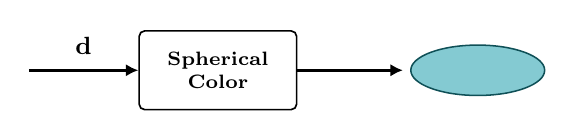
\begin{tikzpicture}[
  font=\sffamily\footnotesize,
  >={Latex[length=4.5pt,width=4.5pt]},
]
\definecolor{cCyan}{HTML}{1F9FAE}   % cyan surfel

% ---------- box ----------
\node[draw=black, line width=0.6pt, rounded corners=2pt,
      fill=white, minimum width=20mm, minimum height=10mm,
      align=center, font=\rmfamily\bfseries\scriptsize] (svBox) at (3.0, 0.0)
  {Spherical\\Color};

% ---------- single viewdir arrow d -> box ----------
\coordinate (dStart) at (0.6, 0.0);
\draw[black, line width=0.9pt, ->]
  (dStart) -- (svBox.west);
\node[font=\sffamily\small, anchor=south]
  at ($(dStart)!0.5!(svBox.west) + (0, 0.08)$) {$\mathbf{d}$};

% ---------- box -> surfel ----------
\coordinate (surfelC) at (6.30, 0.0);
\draw[black, line width=0.9pt, ->]
  (svBox.east) -- ($(surfelC) + (-0.95, 0)$);

% ---------- horizontal cyan surfel (same proportions as scene_intersect) ----------
\begin{scope}[shift={(surfelC)}]
  \filldraw[fill=cCyan!55!white, draw=cCyan!50!black, line width=0.55pt]
    (0,0) ellipse [x radius=0.85, y radius=0.32];
\end{scope}

\end{tikzpicture}
\end{document}
